%
%  Chapter:  3 - 135Pr Experimental Methods
%  Modified: 2/16/2015
%  Author:   James Till Matta
%
%%%%%%%%%%%%%%%%%%%%%%%%%%%%%%%%%%%%%%%%%%%%%%%%%%%%%%%%%%

\chapter{EXPERIMENTAL METHODS}
\label{chp:exp-pr}
Across all of experimental physics there is a common theme in the design of an experiment. Finding a way of producing the system to be studied is one part of this theme. The other part is having the equipment to collect the signals necessary to understand what the system is doing. In nuclear physics, the appropriate choice of reaction will create the desired system and the equipment for signal collection will depend greatly on what one wishes to measure. This chapter will discuss the reaction, detectors, and techniques used in the examination of transverse wobbling in \pr{}.
\section{Heavy-ion Fusion-evaporation Reaction}
\label{sec:exp-pr-fus-evap}
Across nuclear physics there are vast array of reactions used. Narrowing to in-beam \gr{} spectroscopy one finds some common ``workhorse'' reactions that are commonly used. Of these workhorse reactions the heavy-ion fusion-evaporation reaction is frequently chosen for its selectivity in final products, producing relatively few species with large cross-section, and its creation of states with a large amount of angular momentum.\cite{beausang1996arrays}.
\subsection{Creation and Decay of the Compound Nucleus}
\label{ssec:exp-pr-fus-evap-cn}
The fusion evaporation reaction proceeds by the formation of a highly excited compound nucleus, a mechanism first proposed by Neils Bohr\cite{bohr1936neutron}. While it is possible for a compound nucleus to be formed for beam energies below the coulomb barrier the probability is dramatically lower as the beam must quantum mechanically tunnel through same barrier. Therefor for heavy ion fusion to be experimentally feasible the center of momentum energy must exceed the height of the coulomb barrier. The coulomb barrier height can be estimated with

\begin{equation}
\label{eqn:cb_en}
E_{CB}=\frac{\alpha \hbar c Z_p Z_t}{1.16 fm (A_p^{1/3} + A_t^{1/3} + 2)}
\end{equation}

and the non-relativistic limit the center of momentum energy is

\begin{equation}
\label{eqn:cmf_en}
E_{cm} = \frac{\mu}{A_{t}}E_{p}
\end{equation}

Here the subscripts $p$ and $t$ denote projectile and target respectively, $A$ is the mass number, $Z$ represents the nuclear charge, $\alpha{}$ is the fine structure constant, and $\mu = A_{p}A_{t}/(A_{p}+A_{t})$ is the system's reduced mass. After its formation the compound nucleus will have an excitation energy of

\begin{equation}
\label{eqn:cn_ex}
E_{ex} = Q + E_{cm}
\end{equation}

where $Q$ is the reaction's $Q$-value which is,

\begin{equation}
\label{eqn:cn_form_qvalue}
Q = (M_t+M_p-M_{CN})c^2
\end{equation}

The compound nucleus will also carry an angular momentum ranging between $0 \hbar$ and $l_{max} \hbar$, corresponding to head on and peripheral collisions respectively. $l_{max}$ can be estimated classically as

\begin{equation}
\label{eqn:cn_lmax}
l_{max} = \frac{\sqrt{2\mu(E_{cm}-E_{CB})}}{4}(A^{1/3}_p + A^{1/3}_p)\hbar
\end{equation}

, followed by either fissioning of the compound nucleus, or the evaporation of particles, finally leaving behind the excited residual nucleus. In the particle evaporation process each particle must penetrate a barrier, for neutrons this barrier is merely the centrifugal barrier while charged particles see the coulomb barrier added on top of that, this makes neutron emission more probable. Each successive evaporated particle carries energy away from the nucleus until there is insufficient excitation energy for particles to penetrate the emission barrier and the nucleus is left in a state that is stable against particle emission. From this point on the nucleus must dissipate its excess angular momentum and excitation energy via \gr{} emission. A schematic of a (HI, $p3n\gamma{}$) reaction is shown in Fig. \ref{fig:chp3-fus-evap-schem}.
\begin{figure}
	\centerline{\includegraphics[width=\textwidth]{./img/c3/fusion_evaporation_horizontal.pdf}}
	\caption{Schematic illustration of heavy-ion fusion-evaporation, adapted from Ref. \cite{gsBooklet}.}
	\label{fig:chp3-fus-evap-schem}
\end{figure}

\subsection{Choice of Beam and Target}
\label{ssec:exp-pr-fus-evap-beam-target}
When choosing the beam and target for a fusion evaporation one must find the best compromise for 
\subsubsection{Channel Selection}
\label{sssec:exp-pr-fus-evap-beam-target-channel}
\subsubsection{PACE4}
\label{sssec:exp-pr-fus-evap-beam-pace4}

\section{Gamma-ray Spectroscopy}
\label{sec:exp-pr-gamma-spec}
\subsection{Gamma-ray Interaction with Matter}
\label{ssec:exp-pr-gamma-spec-interactions}
As mentioned earlier, the choice of equipment will vary with which signals you need to collect to understand the system. In the case of a residual nucleus at high spin one of the obvious signal choices is the \gr{}s it emits. Detection of gamma-rays is dependent on the \gr{} depositting energy in a detector which in turn depends on the interactions of electromagnetic radiation with matter. At the energies relevant to nuclear physics, $10keV<E_{\gamma}<15MeV$, there are three primary processes to be considered, photoelectric absorption, Compton scattering, and pair production. These three processes compete with each dominating in a different energy range.

\begin{figure}
	\centerline{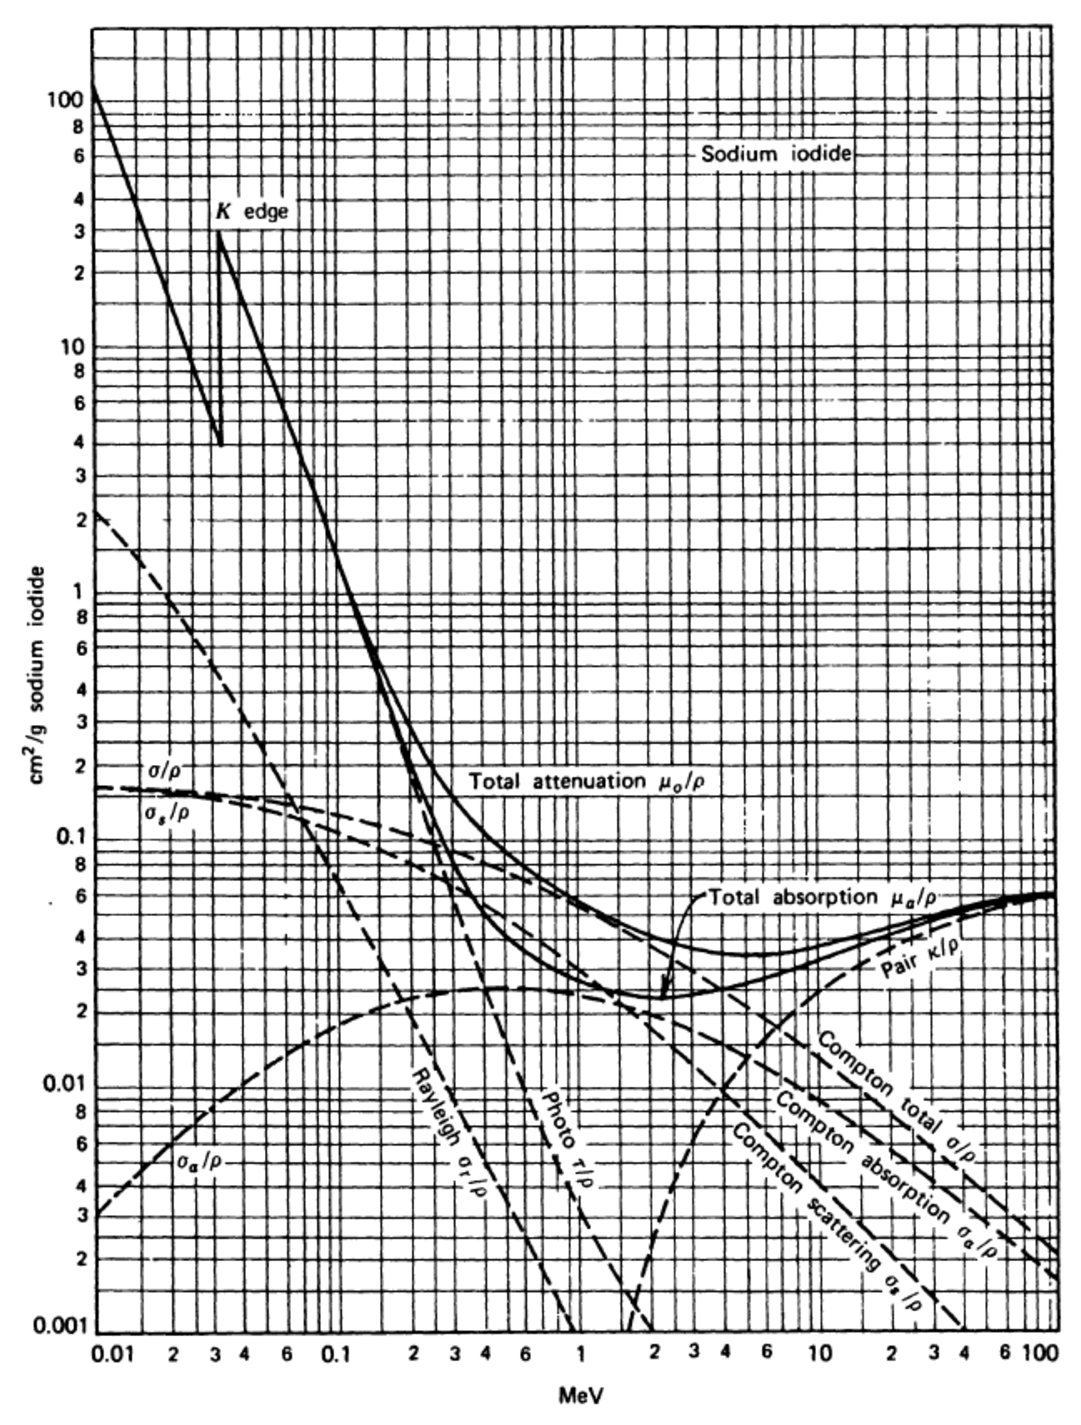
\includegraphics[height=0.65\textheight]{./img/c3/gamma_interactions_scan.eps}}
	\caption{Gamma-ray attenuation coefficients for various processes in NaI, adapted from Ref. \cite{knollBook}. Here we can see the dominance of photoelectric absorption at lower energies, Compton scattering at intermediate energies and pair production at high energies. While the slopes of these processes changes from material to material the trends remain the same.}
	\label{fig:chp3-gamma-interactions}
\end{figure}

In photoelectric absorption the photon interacts with a bound electron in the detector material and is fully absorbed\cite{einstein-PE}. The total energy of the photon is then used to overcome the binding energy of the electron and to provide the electron with kinetic energy, giving $E_{e^-}=E_{\gamma}-E_b$. The electron then proceeds to lose energy as it passes through the detector material. In \gr{} spectra the full energy peak corresponds to the deposition of the photon's full energy in the detector medium. For that to occur either the primary photon, or all the secondary photons (generated by the processes below), must undergo photoelectric absorption. As can be seen in Fig. \ref{fig:chp3-gamma-interactions} the photoelectric effect is dominant at low energies and the energy at which the photoelectric effect ceases to dominate increases with the Z of the material.

In Compton scattering, a \gr{} photon scatters from an electron in the material at some angle $\theta$ to its original direction\cite{Compton-PhysRev.21.483}. Due to conservation of momentum and energy, the energy transferred to the electron is precisely determined by $\theta$ and so the energy of the secondary photon can be written as: $E_{s}=E_{p}(1+\frac{E_{p}}{m_{e}c^2}(1-Cos\theta))^{-1}$ As above the electron then deposits its kinetic energy in the medium as it slows. However, unlike in the photoelectric effect, not all of the energy is deposited in the electron. After the scattering the secondary photon travels in its new direction and is free to interact again with probabilities dictated by its energy. As shown in Fig. \ref{fig:chp3-gamma-interactions} Compton scattering is the dominant effect at intermediate energies.

The final process to be considered is pair production. In pair production the photon enters the region of very strong electric field near the nucleus and its energy is converted into the mass and kinetic energy of an electron positron pair \cite{anderson-PhysRev.43.491,oppenheimer_PhysRev.44.53.2}. Since energy is conserved the photon must have energy of at least twice the rest mass of the electron, giving a threshold of $E_{\gamma}\geq1.022MeV$ for this interaction, any energy above this threshold is converted into kinetic energy shared between the two particles. After their production the electron and positron will both travel through the detector medium loosing energy as they travel. Once at rest the positron will annihilate with an electron, emitting two anti-parallel $511keV$ secondary photons. Fig. \ref{fig:chp3-gamma-interactions} shows the dominance of this interaction at high gamma energies, the energy at which pair production supersedes Compton scattering decreases with increasing Z of the material.

\subsection{High Purity Germanium (HPGe) Detectors}
\label{ssec:exp-pr-gamma-spec-hpge}
In detecting gamma-rays there are essentially 3 major classes of detector, scintillator, gas, and semiconductor detectors. In all cases the \gr{} enters the active volume of the detector and deposits energy by at least one of the processes mentioned above, the primary energetic electrons, produced directly by the interactions of the \gr{}, then proceed to ionize or excite other electrons in the material, the secondary electrons are then detected in some manner. In scintillators they cause UV or visible light to be emitted and that is collected via photomultiplier or similar to produce a voltage pulse. In gas and semiconductor detectors the charge of the secondary electrons (and their corresponding ions or holes) is collected directly, albeit via different mechanisms, to produce the voltage pulse.

It is desirable that \gr{} detectors have both good detection efficiency and energy resolution. Unfortunately, in the \gr{} detectors presently available there is a conflict between these goals and so one must decide which parameter is more important. For high spin experiments where the spectrum is dense with peaks the energy resolution is the top priority as broad peaks would be indistinguishable from each other. Amongst the available detectors, semiconductor detectors, particularly High Purity Germanium (HPGe) detectors offer the best energy resolution.

\begin{figure}
	\centerline{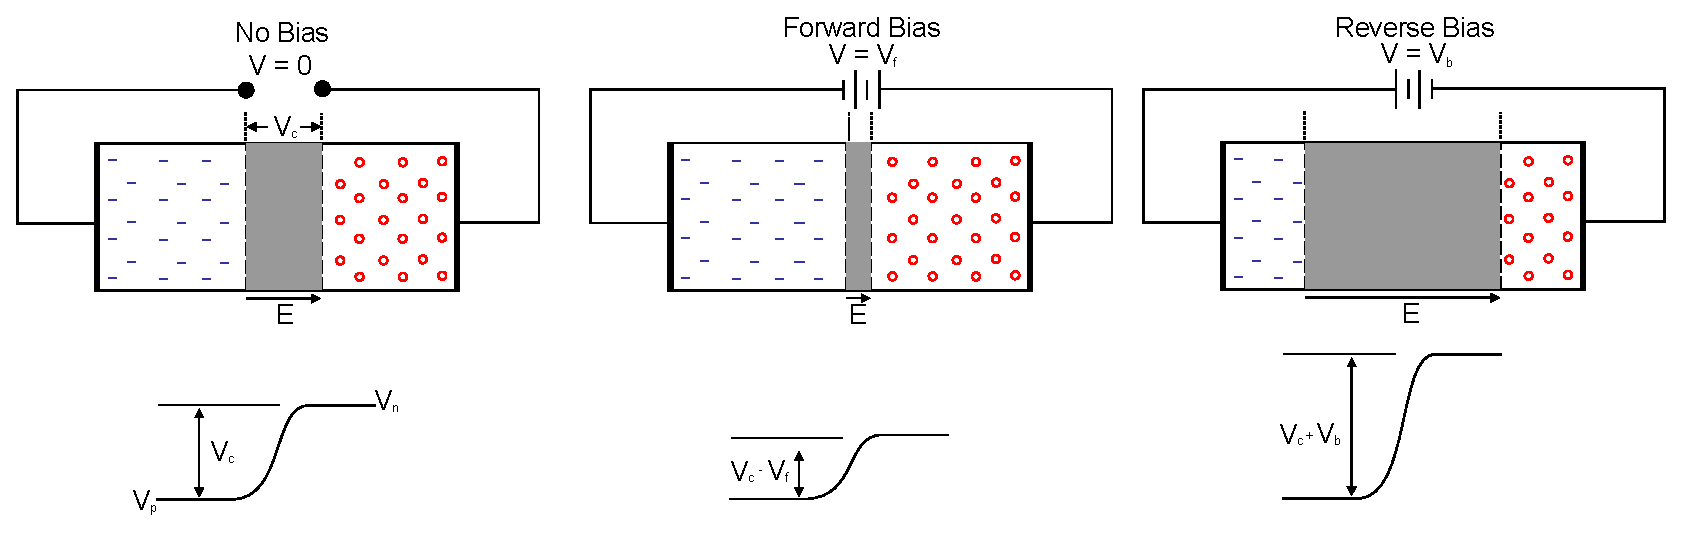
\includegraphics[width=\textwidth]{./img/c3/pn-diode.eps}}
	\caption{Above: Diagramatic view of the depletion zone's with varying bias voltage. Below: Voltage difference across the depletion zone for each bias voltage shown above}
	\label{fig:chp3-pn_diode}
\end{figure}


Semiconductor detectors are reversed bias diodes with either a p-n or a p-i-n junction. At the boundary between the types of materials there is a so called contact potential. This potential gives rise to an electric field which causes the migration of charges between the two materials until there is an area bridging the boundary called the depletion zone. In this zone there is an electric field which gives rise to a potential that counters the contact potential. By applying reverse bias to the diode the contact potential is effectively increased causing the depletion zone to expand (schematic in Fig. \ref{fig:chp3-pn_diode}.) This is desirable because the depletion zone(s) are the only regions of the semiconductor where an electric field will exist. This means that electron hole pairs formed in the within it are swept away from each other before they can recombine so that they can be collected. In contrast, electron hole pairs formed outside the depletion zone are not pulled away from each other and recombine, preventing their collection. Due to this, the depletion zone of the detector is the region that is active. That is to say that the passage of ionizing radiation through the that region is detectable as electron hole pairs it produces will be collected.

The higher the purity of the semiconductor, the higher the reverse bias voltage that can be applied without reaching the breakdown of the semiconductor (usually catastrophic event.) In HPGe detectors the purity is sufficiently high that the whole crystal of Ge can be depleted yielding a very large active region, an advantage for \gr{}s given their low interaction probabilities compared to charged particles. When a gamma interacts in an HPGe detectors it produces at least one high energy secondary electron or positron (more if there are multiple interactions). These secondary electrons lose energy quickly as they pass through the detector, leaving a trail of electron hole pairs in their wake. The electrons and holes are then swept to their respective contacts by the applied potential and collected.

A detectors resolution is defined the FWHM for a given peak. The intrinsic resolution of a semiconductor detector stems from statistical fluctuations in how many electrons and holes are collected at the terminals. As these fluctuations arise from simple counting statistics one their form can be deduced to be:
\begin{equation}
\label{eqn:hpge-res-est} 
\Delta{}E_{in} \propto \frac{E_{\gamma}}{\sqrt{N}}
\end{equation}
Where N is the number of charge carriers produced and is approximately $E_{\gamma}/\epsilon$ where $\epsilon$ is the average energy to make an electron hole pair ($2.96eV$ for Ge). In a more careful examination we see that the intrinsic component of the FWHM is:
\begin{equation}
\label{eqn:hpge-in-res} 
\begin{split}
\Delta{}E_{in}(E) & = 2\sqrt{2 Ln(2)}\frac{E_{\gamma{}}F}{\sqrt{E_{\gamma{}}/\epsilon{}}}\\
       & = 2.355\sqrt{F\epsilon{}E_{\gamma{}}}
\end{split}
\end{equation}
Here $F$ is the Fano factor. This value, intrinsic to the detector material, ranges across $(0,1]$ and takes into account energy loss mechanisms available to the secondary electron(s) that do not generate electron hole pairs. The inquiring reader can find a more thorough explanation in Refs. \cite{knollBook,fano_factor1}.

Unfortunately, the detector's intrinsic resolution is not the only contributor to the detector's resolution. There are also contributions from such sources as electronic noise, charge carrier collection / trapping, and Doppler broadening. If one assumes that these components are independent and normally distributed one gets the actual resolution to be:
\begin{equation}
\label{eqn:hpge-res} 
\Delta{}E_{T}^2 = \Delta{}E_{in}^2 + \Delta{}E_{E}^2 + \Delta{}E_{C/T}^2 + \Delta{}E_{D}^2
\end{equation}
Where $\Delta{}E_{E}$ is the electronic noise contribution, $\Delta{}E_{C/T}$ is the charge collection / trapping term, and $\Delta{}E_{D}$ is the Doppler broadening term. Ref. \cite{trappingResolution} gives the FWHM forms of the noise and collection / trapping terms to be:
\begin{equation}
\label{eqn:hpge-res-noise} 
\Delta{}E_{E} = N_{1/2}
\end{equation}
\begin{equation}
\label{eqn:hpge-res-ct} 
\Delta{}E_{C/T} = 2.355\sqrt{\epsilon{} K E_{\gamma{}} [1-\eta{}(r)]}
\end{equation}
Where $N_{1/2}$ is the FWHM of the electronic noise, $K$ is a constant of a given detector, and $\eta{}(r)$ is the total charge collection efficiency of electrons and holes of the detector as a function of the interaction site's radius.

\begin{figure}
	\centerline{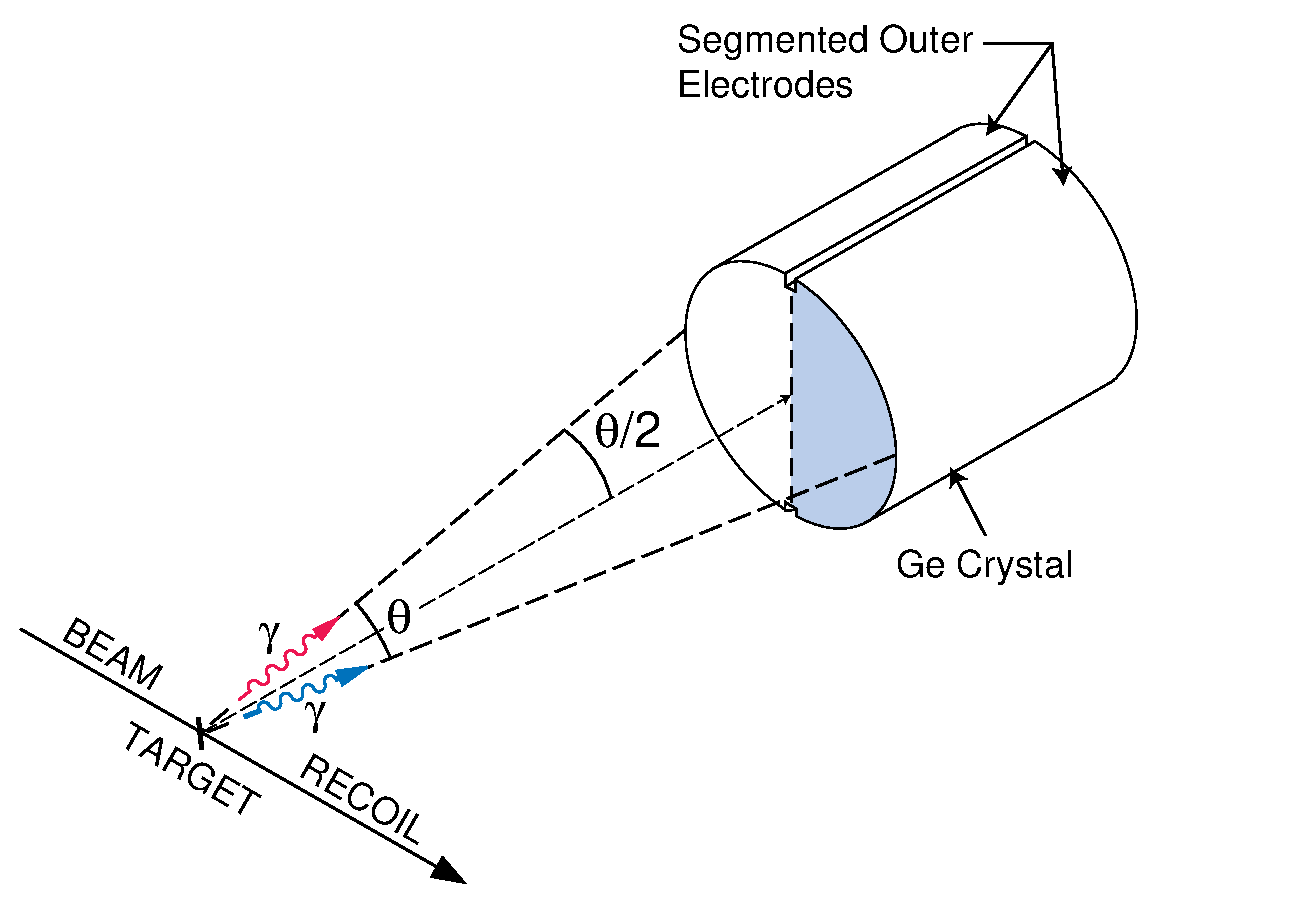
\includegraphics[height=0.3\textheight]{./img/c3/split_contact.eps}}
	\caption{Diagram showing the uncertainty inherent in the \gr{}'s angle of emission, as well as Gammasphere's segmented electrode scheme to reduce this.}
	\label{fig:chp3-doppler-split-contact}
\end{figure}

The final term, $\Delta{}E_{D}$, of this equation comes from uncertainty in the angle at which the gamma ray was emitted from the recoiling nucleus due to the detectors finite size (shown in Fig. \ref{fig:chp3-doppler-split-contact}. The shift in gamma energy due to the nuclear recoil is:
\begin{equation}
\label{eqn:doppler_formula} 
E_{o} = E_{e}\frac{\sqrt{1+\beta{}Cos(\theta)}}{\sqrt{1-\beta{}Cos(\theta)}}
\end{equation}
here, the subscripts o and e refer to observed and emitted, $\beta$ is the speed of the recoiling nucleus and theta is the angle between the nucleus' line of a flight and the emitted \gr{}. If the detector has an angular acceptance such that $\theta{}_{0}-\delta{}\theta{}\leq{}\theta{}\leq{}\theta{}_{0}+\delta{}\theta{}$ with $\theta{}_{0}$ the central angle of the detector; we find that, to first order, the contribution of Doppler broadening is:
\begin{equation}
\label{eqn:res-doppler-term} 
\Delta{}E_{D} = 2\beta{}Sin(\theta{})Sin(\delta{}\theta{})E_{\gamma}
\end{equation}
There are two strategies to combat this term. The first is geometrical. By increasing the granularity of the array, either by using more, smaller detectors, or by using more detectors at a longer distance from the source. This in turn would shrink the opening angle of detectors and therefor reduce the Doppler broadening. The second method is electrical in nature, by segmenting the outer contact of the detector, even roughly, one can localize within the detector where the interaction occurred, therefor effectively reducing the opening angle. Gammasphere uses this strategy as shown in Fig. \ref{fig:chp3-doppler-split-contact}. The split outer contact lets one reduce the effective opening angle, $2\delta{}\theta{}$, from $14.9^{\circ}$ to $7.45^{\circ}$ \cite{TheGS}.

\subsection{Escape Suppression with BGO detectors}
\label{ssec:exp-pr-gamma-spec-escape-supress}
The primary contribution to the background in \gr{} spec is the incomplete deposition of energy in the detector. Two of the mechanisms discussed in section \ref{ssec:exp-pr-gamma-spec-interactions} can lead to this. Compton scattering will result in incomplete energy deposition when the secondary photon yielded by the process may escape the HPGe crystal without depositing the rest of its energy. This mode results in a smooth background from the maximum energy transferable to an electron in the process down to zero energy. Pair production will yield incomplete energy deposition when one or both of the photons from the annihilation of the positron escape the detector. This mode results in 2 new peaks forming, the first $511keV$ below the photopeak, corresponding to one annihilation photon escaping, and a second $1022keV$ below the photopeak, corresponding to both escaping.
\begin{figure}[h!]
	\centerline{
\includegraphics[height=0.25\textheight]{./img/c3/BGO_schematic.pdf}}
	\caption{Schematic of BGO escape suppression around an HPGE crystal.}
	\label{fig:chp3-supression-schematic}
\end{figure}
\begin{figure}[h!]
	\centerline{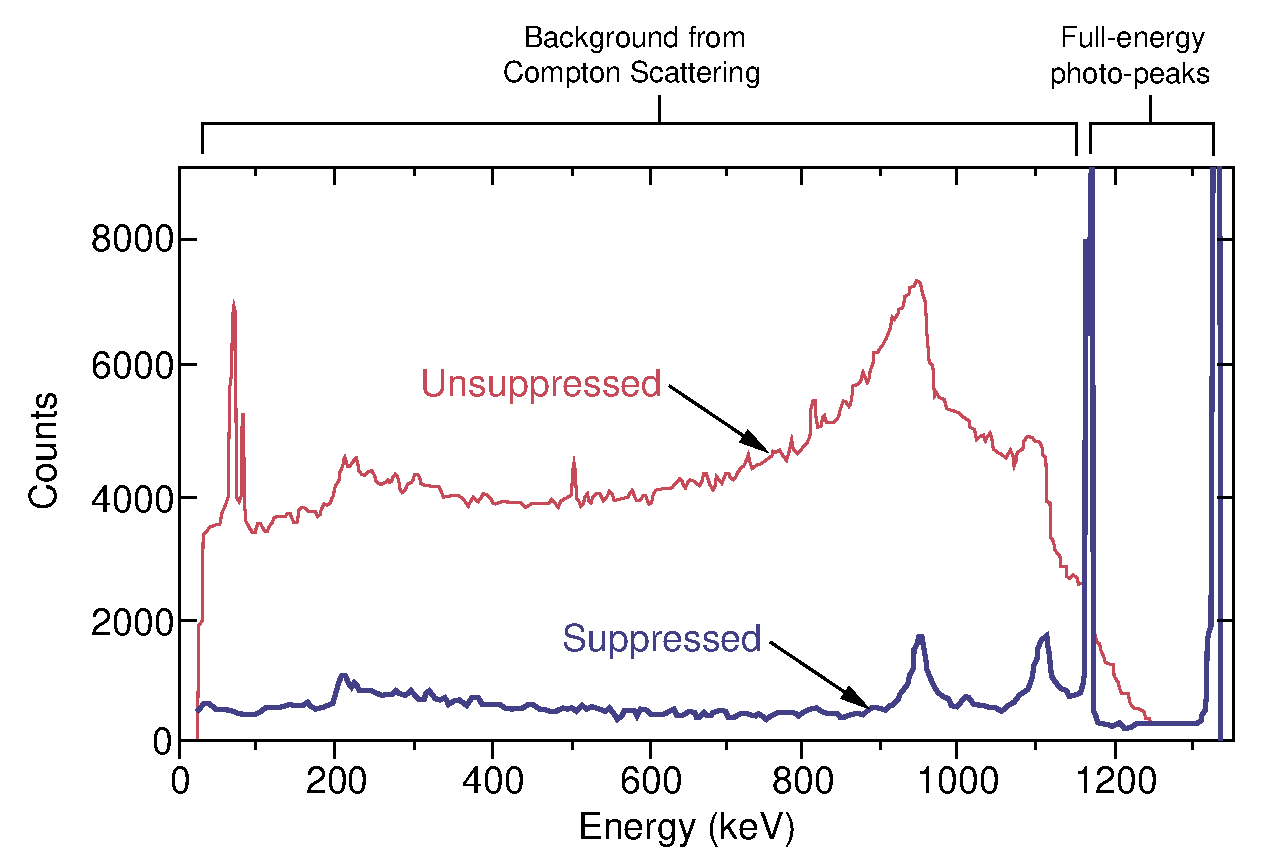
\includegraphics[height=0.25\textheight]{./img/c3/suppressed_spectra.eps}}
	\caption{Superimposed spectra of an escape suppressed and unsuppressed detector. Adapted from Ref.\cite{gsBooklet}}
	\label{fig:chp3-supression-improvement}
\end{figure}
To ameliorate this the principal detector is surrounded by a secondary detector and the electronics are set to be in anti-coincidence (see Fig. \ref{fig:chp3-supression-schematic} for a schematic.) If both detectors had energy deposited, the event is discarded.In practical application, the second detector must be highly efficient at detecting gammas so that it need not be overly large. Given this constraint, the scintillator Bismuth Germanate (BGO) is an excellent choice for escape suppression. While BGO's energy resolution is quite poor, it has excellent timing characteristics, quite high density, and is made of fairly high $Z$ materials. The latter two facts grant it the desired high detection efficiency (substantially higher than the HPGe it is shielding in fact.) Improvements up to a factor of $2.48$ in the peak-to-total ratio (P/T) can be seen for some designs. A bare HPGE detector having a (P/T) of $0.270\pm0.002$ has been see to improve to $0.669\pm0.002$\cite{GSComptonSuppression} with a escape suppression shield around the sides and part of the back (some space needs to be left for cables to exit the HPGe.) Example spectra showing this improvement can be seen in Fig. \ref{fig:chp3-supression-improvement}.

\subsection{The Gammasphere Detector Array}
\label{ssec:exp-pr-gamma-gammasphere}
Gammasphere (partially pictured in Fig. \ref{fig:chp3-gs-hemisphere}) is an array of $110$ escape suppressed HPGe detectors arranged in a sphere around a target. A cross sectional view of part of the array can be seen in Fig. \ref{fig:chp3-gs_det_schem}. The BGO shields are arranged in hexagonal shapes around each detector plus a backplug covering the majority of behind the detector. Gammasphere's spherical geometry is comprised of 17 rings of detectors, each ring at a distinct angle to the beam axis. Using a scheme called honeycomb suppression, Gammasphere has a total efficiency of $~0.09$ at $1MeV$ and a singles P/T of $0.69$.

\begin{figure}[h]
	\centerline{\includegraphics[height=0.3\textheight]{./img/c3/gammasphere_hemi.jpg}}
	\caption{View of scattering chamber and interior of one of Gammasphere's hemispheres drawn back from the chamber. The hexagonal copper foils are x-ray absorbers.}
	\label{fig:chp3-gs-hemisphere}
\end{figure}


\begin{figure}[h]
	\centerline{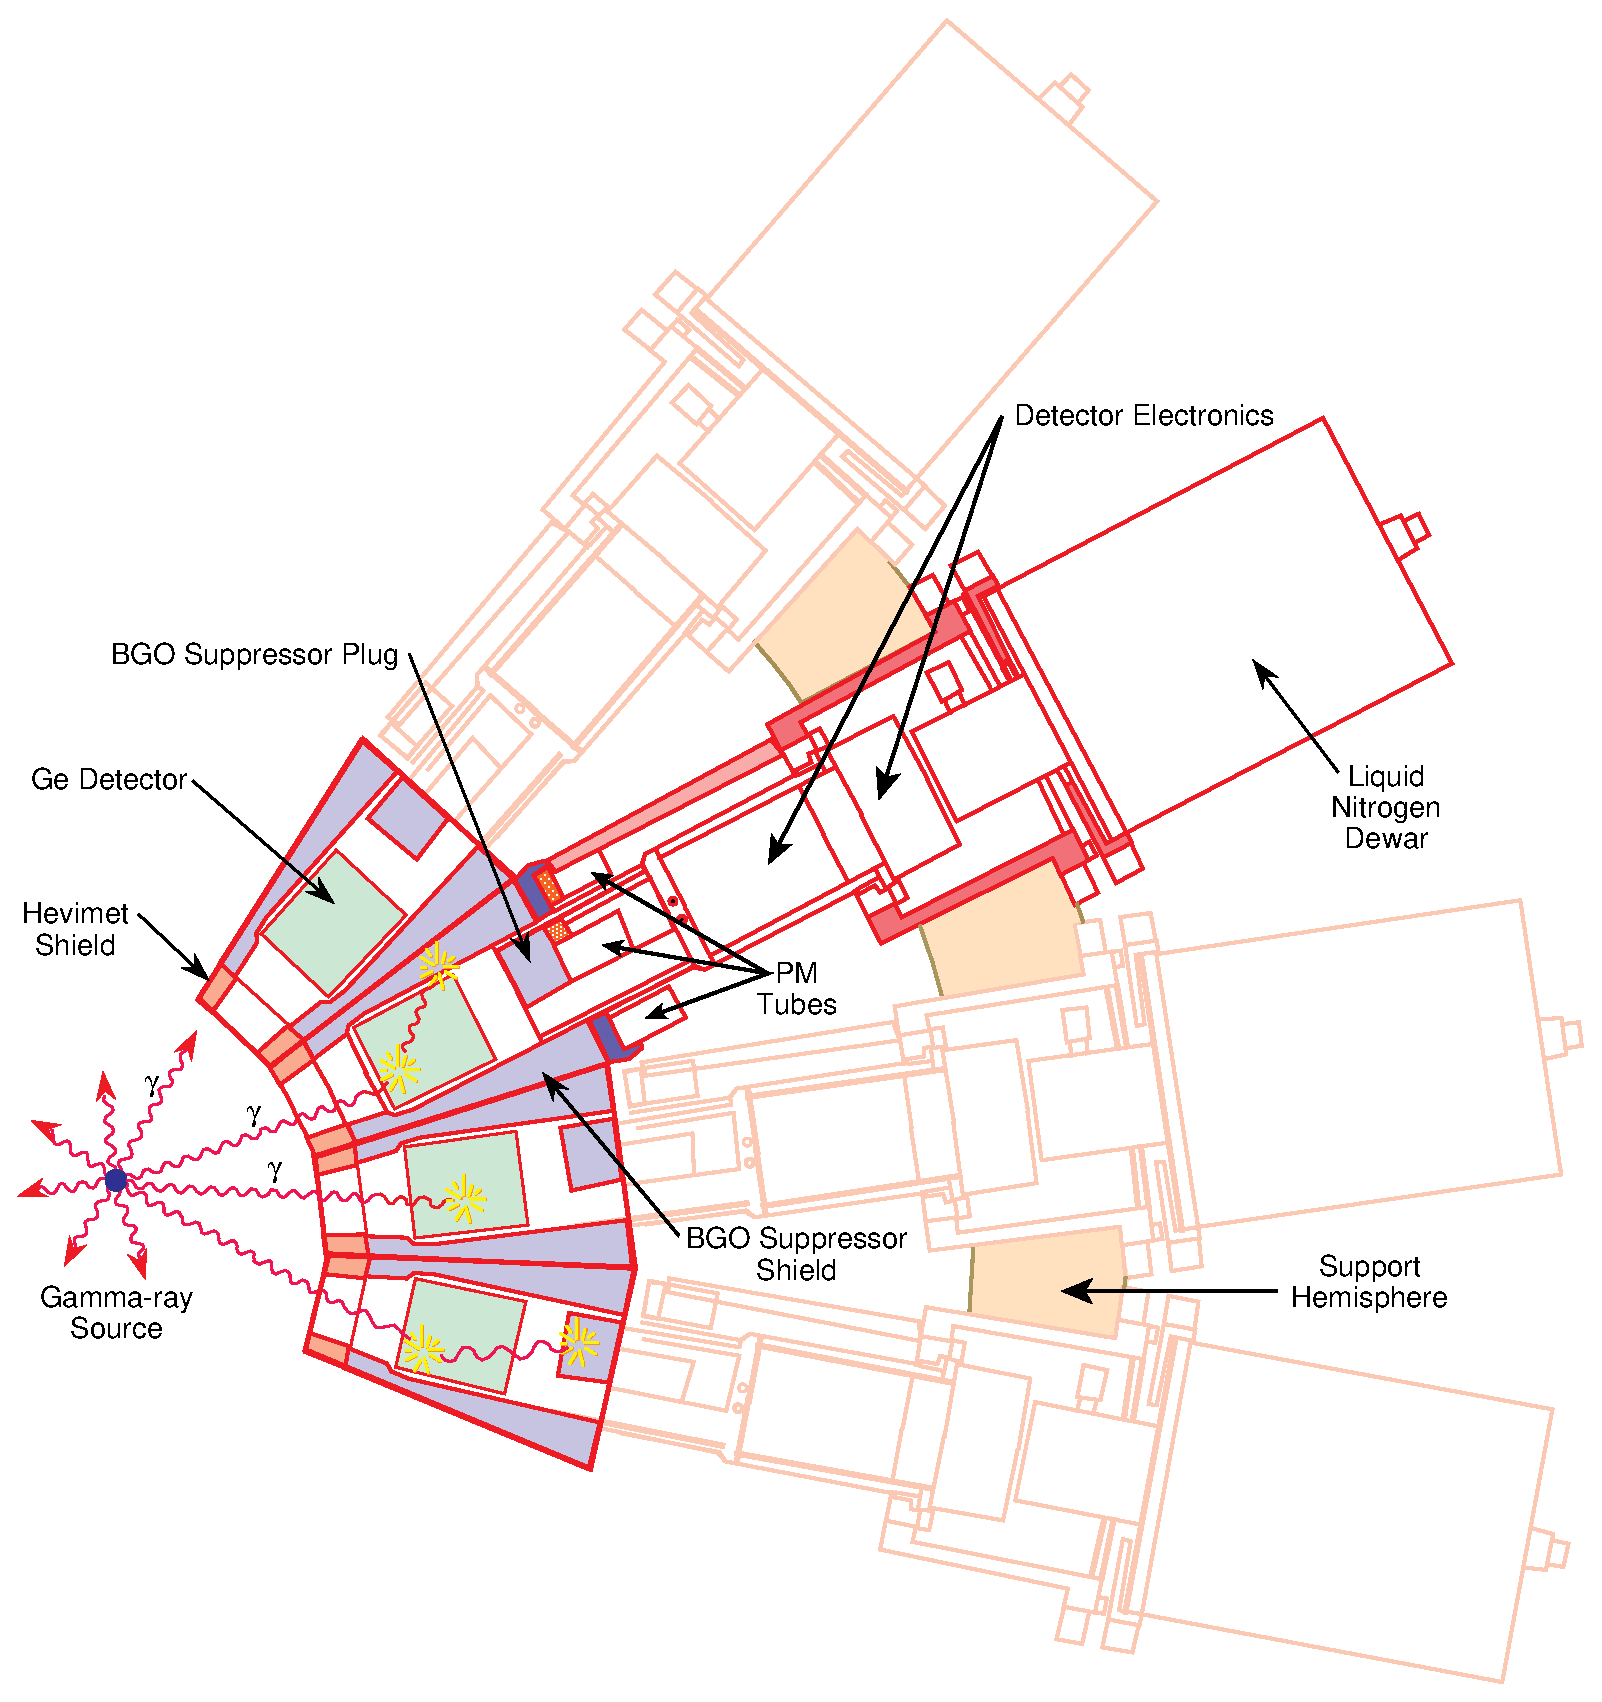
\includegraphics[height=0.3\textheight]{./img/c3/gammasphere_detector.eps}}
	\caption{Cross-section schematic of part of Gammasphere. Adapted from Ref.\cite{gsBooklet}}
	\label{fig:chp3-gs_det_schem}
\end{figure}


Honeycomb suppression is an escape suppression scheme that uses the BGO shields of adjacent detector modules to effectively double the thickness of a detector's shields. As seen in Fig. \ref{fig:chp3-gs_det_schem} almost every module will have additional modules immediately adjacent to it. If the HPGe detector for a given module do not register energy deposition the 6 side segments of its BGO shield are used to double the thickness of the shields they are adjacent to. Without this measure the singles P/T is $\sim0.62$; using honeycomb suppression improves this to $\sim0.69$ though it reduces the total efficiency at 1.332MeV from $\sim0.095$ to $\sim0.089$\cite{TheGS}.

\begin{table}
\begin{center}
\begin{tabular}{|c|c|}
\hline
\hline \multicolumn{2}{|c|}{Gammasphere Feature Summary}  \\ 
\hline No. Detectors             & 110 \\ 
No. Segmented Detectors   & 70 \\ 
HPGe Detector Size        & $7.1$cm (D) $\times$ $8.22$cm (L) \\ 
HPGe Target to Front      & $24.6$cm\\ 
Total HPGE Solid Angle    & $0.46 \times 4\pi$\\ 
Total Peak Efficiency     & $0.094$ at $1.3 MeV$\\ 
Singles P/T               & $0.6$ at $1.3 MeV$ \\ 
Energy Resolution (MeV)   & $2.1keV$ at $1.3 MeV$ \\ 
\hline 
\hline 
\end{tabular}
\end{center}
\caption{Summary of Gammasphere features and characteristics, drawn from Refs. \cite{TheGS,SimulatedResGS,GSComptonSuppression,largeArrays}}
\label{tbl:gs-summary}
\end{table}

As mentioned in section \ref{ssec:exp-pr-gamma-spec-hpge} some of Gammasphere's detectors have a split outer electrode to reduce the effective half angle. Detector positions can be found in table \ref{tbl:app1-gs-rings} and table \ref{tbl:app1-gs-detectors} in appendix \ref{app:gs-rings-and-detectors}. Table \ref{tbl:gs-summary} contains a brief summary of Gammasphere's features. Gammasphere's high granularity, good energy resolution, and efficiency make it a boon to high spin coincidence measurements where the \gr{} multiplicity is high.

\subsection{Indian National Gamma Array (INGA)}
\label{ssec:exp-pr-gamma-spec-inga}

\section{Experimental Details}
\label{sec:exp-pr-details}
\subsection{ATLAS/Gammasphere}
\label{ssec:exp-pr-details-gs}
\subsection{TIFR - BARC Pelletron LINAC / INGA}
\label{ssec:exp-pr-details-inga}

\section{Data Processing}
\label{sec:exp-pr-data-proc}
\subsection{Calibration}
\label{ssec:exp-pr-data-proc-cal}
\subsection{Background Subtraction}
\label{ssec:exp-pr-data-proc-bg-sub}
\subsubsection{Symmetric Gates}
\label{sssec:exp-pr-data-proc-bg-sub-sym}
\subsubsection{Asymmetric Gates}
\label{sssec:exp-pr-data-proc-bg-sub-asym}

\section{Angular Distributions, Correlations, and Polarization}
\label{sec:exp-pr-data-ang}
\subsection{Angular Distributions}
\label{ssec:exp-pr-data-ang-dist}
Testing 1
\subsection{Angular Correlations}
\label{ssec:exp-pr-data-ang-cor}
Testing 2
\subsubsection{Directional Correlation of Gamma-rays from Oriented Nuclei DCO Ratios}
\label{sssec:exp-pr-data-ang-cor-dco}
Testing 3
\subsection{Polarization}
\label{ssec:exp-pr-data-ang-pol}
Testing 4
